% !TeX root ../../tgame_doc
% !TeX spellcheck = en_GB

Even though in principle one could produce interactive objects using context methods denoted as private, the recommended way is to always define object whose instance are supposed to actively interact with the user and the environment through the appropriate choice of decorators. For user not familiar with this Python feature they can simply be though as tag that provide extra methods out of the box.\\
In principle more than one decorator can be used at once, however it's important to understand that some of them implicitly call others or conversely need others to be called before. Below is a comprehensive dependencies graph (red node denotes decorator that will be introduced in future versions)

\begin{center}
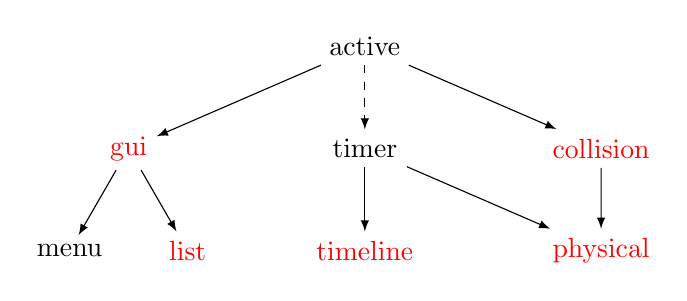
\begin{tikzpicture}[yscale = 0.65, xscale = 0.75]
	\node (active) at (0, 10) {\code{active}};
	\node (gui) at (-4, 8) {\color{red}\code{gui}};
	\node (timer) at (0, 8) {\code{timer}};	
	\node (collision) at (4, 8) {\color{red}\code{collision}};
	\node (timeline) at (0, 6) {\color{red}\code{timeline}};
	\node (menu) at (-5, 6) {\code{menu}};
	\node (list) at (-3, 6) {\color{red} \code{list}};
	\node (physical) at (4, 6) {\color{red} \code{physical}};
	
	
	\draw[-latex] (active) to (gui);
	\draw[-latex] (gui) to (menu);
	\draw[-latex] (gui) to (list);
	\draw[-latex, dashed] (active) to (timer);
	\draw[-latex] (timer) to (timeline);
	\draw[-latex] (active) to (collision);
	\draw[-latex] (collision) to (physical);
	\draw[-latex] (timer) to (physical);
\end{tikzpicture}
\end{center}